\documentclass[10pt,twocolumn]{article}

\usepackage[a4paper,margin=2.1cm]{geometry}
\usepackage[utf8]{inputenc}
\usepackage[T1]{fontenc}
\usepackage{times}
\usepackage{graphicx}
\usepackage{booktabs}
\usepackage{amsmath}
\usepackage{url}
\usepackage[hidelinks]{hyperref}
\usepackage{caption}
\captionsetup{font=small,labelfont=bf}

\title{\vspace{-1.2cm}\bfseries YOLOJ: Where a Vision--Language Model Looks\\
When It Answers Yes or No}

\author{%
Samuel Otero Agraso\\
\small\url{https://github.com/XxSamaxX/YOLOJ}
}
\date{}

\begin{document}
\maketitle

\begin{abstract}
\noindent
A \emph{semantic if} reads a yes/no decision from the answer-token logits of a
language model in one forward pass. We ask whether the same forward pass can
also say \emph{where}: whether a vision--language model that answers ``is there
a remote control?'' can be turned into a detector for a predicate declared at
run time, with no detection head, no label set and no training.

The obvious construction, a YOLO-like pyramid of crops with one predicate per
cell, localises correctly but costs 8--16\,s per image on a 27B model. Looking
inside Qwen3-VL-4B instead, we find that the decision appears at layer 24 of
36, that the model attends to the image in layers 17--23, that one fixed patch
absorbs 65--78\% of the late attention regardless of the question, and that a
handful of heads in layers 20--22 point at the object once that sink is divided
out with the attention map of a content-free question. Five heads chosen on 200
COCO images hit the object on 78.5\% of 200 held-out images in the pointing
game (chance 10.6\%, image centre 29.0\%, mean of all heads 1.5\%); the logit
gap separates present from absent categories at AUC 0.996, and its sign is
already settled at layer 24. Sharing the image prefix across questions brings
each further predicate down to 12--17\,ms, so all 80 COCO classes cost 1.2\,s.

Turning the point into a mask is where the approach stops being competitive.
Prompting SAM 2.1 or SAM 3 with the peak gives 54.5--59.5\% of boxes with
IoU\,$\geq$\,0.5; floating-point precision, one mask per peak and removing
stray fragments do not help. SAM 3 prompted with the category \emph{name} and
no language model at all reaches 85.0\%, finds 83.2\% of individual instances
against 35.0\%, and separates present from absent at AUC 0.990. For anything
that has a name, a concept segmenter is the better localiser.

What the segmenter does not do is judge. On a single photograph, its scores
for ``man with open mouth'' and ``man with closed mouth'' are 0.30 and 0.54 and
it scores ``sleeping man'' at 0.47, while the logit gap answers the same
questions with margins of 16--29 nats. We therefore argue for a division of
labour---the language model decides, the segmenter delineates---report a
5\,Hz live demonstration and a first test on desktop screenshots, and state
plainly which of these claims are measured and which rest on one image.
\end{abstract}

\section{Introduction}

Open implementations of the \emph{semantic if} \cite{semif,jevcpu} turn a
language model into a conditional defined at run time: the question is posed
with lettered options, a single forward pass is run, and the decision is the
difference between the logits of the two letters. Ported to a vision--language
model, the readout answers perceptual questions about an image in about
90\,ms \cite{discern}. It says whether, not where.

Detectors of the YOLO family \cite{redmon2016yolo} say where, for a vocabulary
fixed at training time; open-vocabulary detectors
\cite{cheng2024yoloworld,liu2024groundingdino} relax the vocabulary to noun
phrases. A semantic if accepts any predicate that can be written as a
question---a state, a relation, a reading of text---so a detector built on it
would localise things that have no class name. This paper reports an attempt
to build one, YOLOJ, on a single consumer GPU, and is as much about where the
attempt loses as about where it works.

The contributions are measurements:

\begin{itemize}\setlength{\itemsep}{0pt}
\item A dissection of where Qwen3-VL-4B decides a yes/no question and where it
looks while doing so, including an attention sink that hides the useful
signal when heads are averaged (Section~\ref{sec:inside}).
\item A held-out evaluation on COCO of training-free localisation from five
attention heads, and of presence and early exit from the logit gap
(Section~\ref{sec:coco}).
\item A shared-prefix scheme that makes additional predicates on the same
image cost 12--17\,ms (Section~\ref{sec:prefix}).
\item Three negative results on converting the attention peak into a mask,
and a direct comparison in which SAM 3 prompted by text clearly beats the
whole chain on named objects (Sections~\ref{sec:mask}--\ref{sec:sam3}).
\item Small-scale evidence on what remains for the language model: states,
live video and screenshots (Section~\ref{sec:niche}).
\end{itemize}

\section{Related work}

\textbf{Reading decisions from logits.} SemIf \cite{semif} and JEV-CPU
\cite{jevcpu} read a decision from answer-token logits; \texttt{discern}
\cite{discern} carries the readout to images and studies the logit gap as a
confidence signal. We reuse its prompt contract unchanged.

\textbf{Attention as localisation.} Zhang et al.\ \cite{zhang2025mllms} show
that multimodal models attend to the relevant region even when they answer
wrongly, and normalise the attention map by that of a generic instruction
before cropping; our relative map is the same normalisation. Kang et al.\
\cite{kang2025heads} show that a few attention heads suffice for training-free
grounding; we confirm this on a different model and question format and
measure it against a text-prompted segmenter. FastV \cite{chen2024fastv}
observes that image tokens receive little attention in deep layers and prunes
them. The single patch that absorbs most late attention in our measurements is
reminiscent of the artefact tokens described in vision transformers
\cite{darcet2024registers}, although here it is observed in the language
model's attention over image tokens.

\textbf{Segmentation.} SAM \cite{kirillov2023sam} and SAM 2
\cite{ravi2024sam2} segment from points and boxes; SAM 3
\cite{carion2025sam3} adds prompts given as short noun phrases and returns
every instance of the concept. LISA \cite{lai2024lisa} trains a language model
to emit a segmentation token for queries that need reasoning. Nothing in the
present work is trained.

\textbf{Benchmarks.} We use COCO val2017 \cite{lin2014coco} and the pointing
game \cite{zhang2016pointing}. Our absent categories are drawn at random, the
easiest of the negative-sampling settings of POPE \cite{li2023pope}.

\section{Method}

\subsection{Readout}

The model receives a system message, the image, and a JSON object with the
criterion and two options, \texttt{A}: yes and \texttt{B}: no. Generation is
not run: the decision is the gap $g = \ell_A - \ell_B$ between the logits of
the two letters at the first answer position, in nats. A bare object name is
wrapped into a presence question; a full question is passed as written.

\subsection{Pyramid of crops}

The black-box construction evaluates the predicate on the whole image, then on
a $2\times2$ and a $4\times4$ grid of crops, pruning the children of any cell
whose gap falls below $-3$ nats (Figure~\ref{fig:pyramid}). Because the model
leans towards letter \texttt{A} by about 2.4 nats, a cell under 6 nats is asked
again with the options swapped and the two gaps averaged. This needs only an
inference server and was run against Qwen3.8-27B quantised to about 2 bits per
weight.

\begin{figure}[t]
\centering
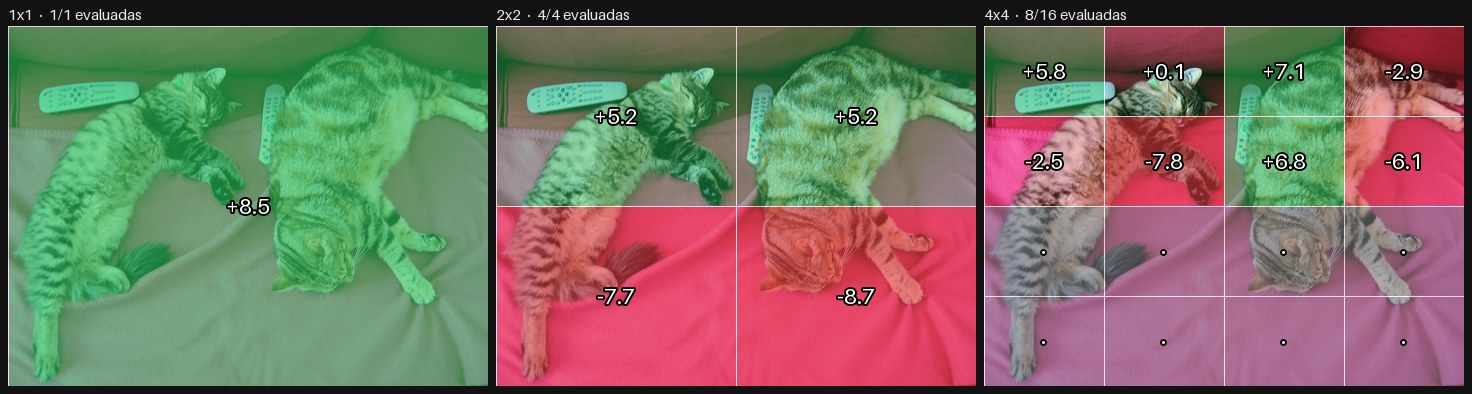
\includegraphics[width=\columnwidth]{figures/pyramid.jpg}
\caption{The pyramid of crops for ``is any part of a remote control
visible?'': 19 forward passes, 7.7\,s. Green is yes, red is no, numbers are
the gap in nats; grey cells were pruned.}
\label{fig:pyramid}
\end{figure}

\subsection{Relative attention of a few heads}

For the white-box route we run Qwen3-VL-4B \cite{qwen3vl} in
\texttt{transformers}, unquantised in bfloat16, on the whole image. Its vision
encoder \cite{siglip2} produces one token per $32\times32$ pixels; the language
model has 36 layers of 32 heads. For a head $h$ we take the attention from the
last prompt position to the image tokens, $a_h(q)$, reshaped to the token grid.
The map for a question $q$ is
\[
m(q) = \sum_{h \in H} \frac{r_h}{\sum r_h}, \qquad
r_h = \frac{a_h(q)}{a_h(q_0) + \epsilon},
\]
where $q_0$ is the content-free question ``Is this an image?'' asked of the
same image, and $H$ is a set of five heads. The map is smoothed with a
$3\times3$ mean and its maximum is the predicted location. The heads are
ranked on a tuning set by how well their map matches the object mask and fixed
thereafter: (layer.head) 20.15, 20.4, 21.18, 21.31 and 22.6.

\subsection{Shared image prefix}
\label{sec:prefixmethod}

Every question about an image shares the start of the prompt, system message
plus image. That prefix is run once and its key/value cache kept; the questions
and $q_0$ are then a batch of suffixes of about 45 tokens each on top of the
cache.

\subsection{From a point to a mask}

The peak of $m(q)$ is handed to SAM as a positive point. Of the three masks SAM
proposes we keep the one whose footprint on the token grid has the highest IoU
with the map thresholded at half its maximum. As an alternative that uses no
language model, SAM 3 is prompted with the category name and its instances
scoring at least 0.5 are kept.

\section{Experimental setup}

All runs use one RTX 3080 with 12\,GB. Images come from COCO val2017. We
sample 400 images with one \emph{present} category whose instances together
cover 0.5--30\% of the image and one \emph{absent} category drawn at random.
The first 200 (half A) are used for every choice---heads, thresholds, number
of peaks---and the other 200 (half B) only for reporting. Unless stated, a
\emph{good box} is one whose IoU with the box of the union of the real
instances is at least 0.5, and results are split by whether the image has one
instance of the category (134 images of half B) or several (66).

The pointing game counts a hit when the peak falls on a grid cell at least a
quarter covered by the object. Chance is the mean fraction of such cells.

\section{Results}

\subsection{The pyramid works and is too slow}

On five predicates over three images the pyramid localises as expected
(Figure~\ref{fig:pyramid}), at 0.7\,s per forward pass on the whole image and
0.37\,s per crop. An absent object costs one forward pass; a present one costs
nearly the full grid, 7.7--15.7\,s, because crop gaps sit under the calibration
threshold. Passing the region as text coordinates instead of a crop localised
poorly. This route was read by eye only and is kept as a reference.

\subsection{Where the answer is made}
\label{sec:inside}

Reading the gap from each layer's hidden state gives noise up to layer 23,
$\pm7$ to $\pm9$ nats with the right sign at layer 24, and $\pm19$ to $\pm22$
at the last layer, in all five first cases. The attention to image tokens
concentrates in layers 17--23, immediately before the decision. From layer 18
on, 65--78\% of that attention goes to one patch that does not change with the
question; averaging heads shows only that patch. A few heads in layers 20--21
nevertheless place 25--76\% of their image attention inside the object, and
their attention mass drops when the object is absent (Figure~\ref{fig:heads}).
A forward pass takes 126\,ms and 8.3\,GiB; returning every layer's attention
adds little.

\begin{figure*}[t]
\centering
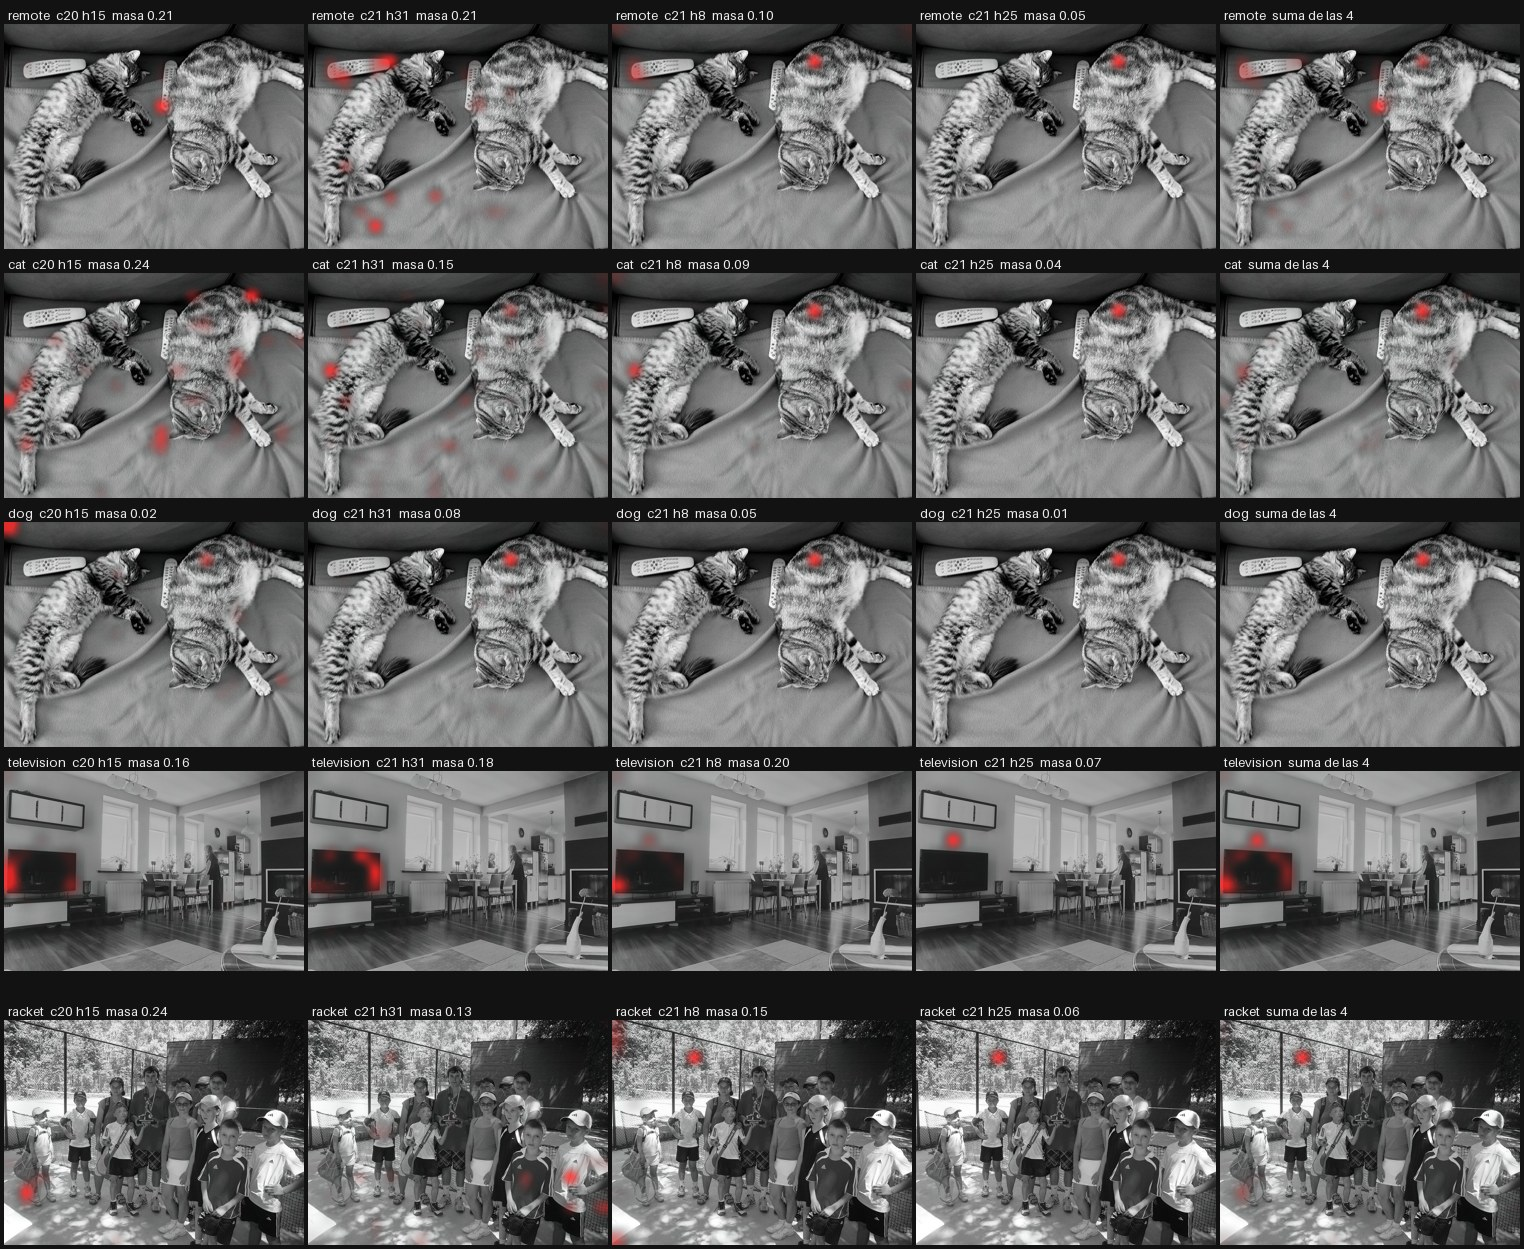
\includegraphics[width=0.86\textwidth]{figures/heads.jpg}
\caption{Raw attention of four heads (columns 1--4) and their sum (column 5)
for five predicates: remote, cat, dog (absent), television, racket. Labels give
layer (c) and head (h) and the attention mass on the image (``masa''). The dot
that persists on the cat's back in the right-hand columns, whatever the
question, is the sink. These heads were picked by eye on two of these images;
the held-out evaluation is in Table~\ref{tab:pointing}.}
\label{fig:heads}
\end{figure*}

\subsection{Held-out localisation on COCO}
\label{sec:coco}

Table~\ref{tab:pointing} and Figure~\ref{fig:pointing} give the pointing game
on half B. Averaging all 1152 heads is worse than chance because of the sink.
The best single head, 20.15, was spotted by eye on two photographs in the first
pass and is also the best on 198 images. Dividing by the map of the
content-free question raises it from 59.5\% to 71.5\%; masking the three
most-attended cells instead gives 59--64\%. Five heads reach 78.5\%.

\begin{table}[t]
\centering\small
\begin{tabular}{lrr}
\toprule
Map & Hit rate & AUC \\
\midrule
Chance (object area) & 10.6\% & 0.500 \\
Centre of the image & 29.0\% & 0.650 \\
Mean of all 1152 heads, raw & 1.5\% & 0.648 \\
Head 20.15, raw & 59.5\% & 0.837 \\
Head 20.15, relative & 71.5\% & 0.880 \\
Five chosen heads, relative & \textbf{78.5\%} & \textbf{0.892} \\
\bottomrule
\end{tabular}
\caption{Pointing game on 200 held-out COCO images. AUC is that of the map as
a per-cell classifier of the object mask.}
\label{tab:pointing}
\end{table}

\begin{figure}[t]
\centering
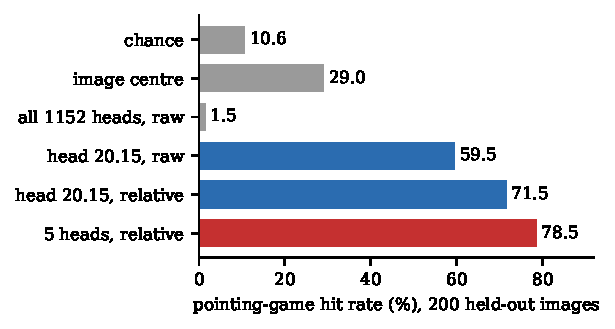
\includegraphics[width=\columnwidth]{figures/pointing.pdf}
\caption{Pointing-game hit rate, held-out half.}
\label{fig:pointing}
\end{figure}

\textbf{Presence.} On the same images the gap at the last layer separates the
present from the absent category at AUC 0.996, and the attention mass of three
chosen heads at 0.992.

\textbf{Early exit.} The gap read at each layer is at chance up to layer 21.
Its sign is correct on 96.5\% of items at layer 24 and on 96.5\% at layer 35;
the remaining layers sharpen the gap (AUC 0.969 to 0.996) without changing its
side. We did not truncate the model to measure the saving.

\subsection{The image once, the questions in a batch}
\label{sec:prefix}

The prefix of system message and image is 338 of about 385 prompt tokens.
Running it once costs 133\,ms (49\,ms of vision encoder, 85\,ms of language
model); a predicate plus $q_0$ on top cost 34\,ms, and each further predicate
12--17\,ms (Table~\ref{tab:prefix}). The answers match those of a plain forward
pass on 30 images by 3 questions: the gap moves by 0.26 nats on average and
1.0 at most, the sign agrees on 90 of 90, and the head maps correlate at 0.99
on average and 0.83 at worst. Batches above 13 questions exhaust the 12\,GB
when attention is returned for every layer.

\begin{table}[t]
\centering\small
\begin{tabular}{lrr}
\toprule
 & Plain & Shared prefix \\
\midrule
Image, predicate and $q_0$ & 259\,ms & 167\,ms \\
Each further predicate & 128\,ms & 12--17\,ms \\
All 80 COCO classes & $\sim$10.5\,s & 1.2\,s \\
\bottomrule
\end{tabular}
\caption{Cost per image at $640\times480$, Qwen3-VL-4B in bfloat16.}
\label{tab:prefix}
\end{table}

\subsection{From the point to a mask}
\label{sec:mask}

Thresholding the attention map alone gives a mask IoU of 0.36 and 42\% of good
boxes: each cell is 32 pixels wide, so the map is a blob by construction.
Table~\ref{tab:sam} gives the result of prompting a segmenter with the peak.
Choosing among SAM's three candidates by agreement with the map beats choosing
by SAM's own score (58.0\% against 48.5\% for SAM 2.1 large). The ceiling, had
the best of the three candidates always been chosen, is 65.5--71.0\%.

\begin{table}[t]
\centering\small
\setlength{\tabcolsep}{3.5pt}
\begin{tabular}{lrrrr}
\toprule
 & Mask & Good & One / & \\
Segmenter (1 point) & IoU & boxes & several & ms \\
\midrule
Attention alone & 0.36 & 42.0\% & 39 / 48 & -- \\
SAM 2.1 small & 0.531 & 54.5\% & 69 / 24 & 21 \\
SAM 2.1 large & 0.553 & 58.0\% & 74 / 26 & 71 \\
SAM 3 (tracker) & 0.549 & 59.5\% & 73 / 32 & 160 \\
\midrule
SAM 2.1 small, float32 & 0.537 & 55.5\% & 71 / 24 & 54 \\
SAM 2.1 large, float32 & 0.553 & 58.0\% & 75 / 24 & 199 \\
SAM 3, float32 & 0.551 & 58.0\% & 73 / 27 & 465 \\
\bottomrule
\end{tabular}
\caption{Attention peak as a point prompt, held-out half, pixel level.
``One / several'' is the percentage of good boxes on images with one instance
of the category and with several. Top block in bfloat16.}
\label{tab:sam}
\end{table}

Three attempts to improve on this failed, and we report them as such.

\textbf{Precision.} Ragged mask borders suggested a half-precision artefact.
Running the segmenters in float32 changes nothing beyond noise and costs
2.6--2.9 times the time (Table~\ref{tab:sam}, lower block).

\textbf{One mask per peak.} Passing each peak of the map as its own object and
joining the masks, with the number of peaks and their threshold chosen on half
A, helps images with several instances (24\% to 30\%) and hurts those with one
(70\% to 66\%): 54.5\% overall against 55.0\%. The eight points it gained on
the tuning half did not carry over.

\textbf{Removing fragments.} At full resolution 39--50\% of the chosen masks
come in more than five connected pieces. Keeping only the piece that contains
the point, or the largest, lowers good boxes by 3--6 points
(Table~\ref{tab:clean}). Images with one instance are unchanged; images with
several lose, because the reference is the union of all instances and the
``stray'' pieces were often the other instances. The fragments are a cosmetic
problem; the instances are the real one.

\begin{table}[t]
\centering\small
\setlength{\tabcolsep}{4pt}
\begin{tabular}{lrrr}
\toprule
Kept & 2.1 small & 2.1 large & SAM 3 \\
\midrule
Everything & 54.5 & 58.0 & 59.5 \\
Piece under the point & 51.5 & 55.0 & 53.5 \\
Largest piece & 51.5 & 55.5 & 53.5 \\
Pieces $\geq$ 10\% of largest & 53.0 & 56.0 & 56.0 \\
\bottomrule
\end{tabular}
\caption{Good boxes (\%) after removing mask fragments, held-out half.}
\label{tab:clean}
\end{table}

\subsection{A concept segmenter does it better}
\label{sec:sam3}

SAM 3 prompted with the category name, with no language model involved, is
compared with the chain in Table~\ref{tab:sam3} and Figure~\ref{fig:boxes}.
Scored against the union it gives 85.0\% of good boxes against 58.0\%, and the
gap between one and several instances disappears (87\% and 82\%). Matching
each real instance one-to-one to a predicted box at IoU\,$\geq$\,0.5, it finds
83.2\% of 386 instances against 35.0\%. On objects under 3\% of the image it
gives 77\% of good boxes against 38\%. Its maximum instance score separates the
present from the absent category at AUC 0.990, against 0.996 for the logit gap.
Figure~\ref{fig:examples} shows two images with several instances.

\begin{table}[t]
\centering\small
\setlength{\tabcolsep}{3.5pt}
\begin{tabular}{lrrrr}
\toprule
 & Good & Instances & Boxes & of them \\
Method & boxes & found & given & correct \\
\midrule
Attention + point & 58.0\% & 35.0\% & 200 & 67.5\% \\
SAM 3 text, $\geq 0.3$ & 81.5\% & 88.9\% & 621 & 55.2\% \\
SAM 3 text, $\geq 0.5$ & \textbf{85.0\%} & 83.2\% & 439 & 73.1\% \\
SAM 3 text, $\geq 0.7$ & 79.5\% & 76.2\% & 345 & 85.2\% \\
\bottomrule
\end{tabular}
\caption{SAM 3 prompted by the category name against the attention chain (SAM
2.1 large), held-out half. Crowd annotations are excluded from the instance
count, which understates the last column.}
\label{tab:sam3}
\end{table}

\begin{figure}[t]
\centering
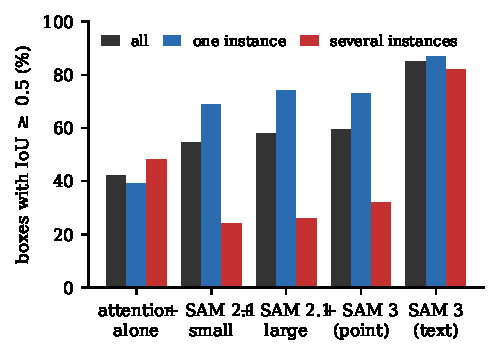
\includegraphics[width=\columnwidth]{figures/boxes.pdf}
\caption{Boxes with IoU\,$\geq$\,0.5 by method and by number of instances of
the category in the image.}
\label{fig:boxes}
\end{figure}

\begin{figure*}[t]
\centering
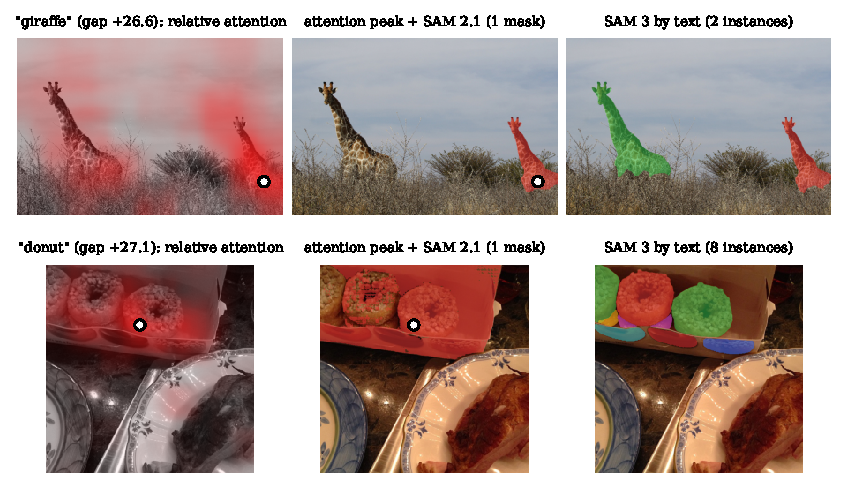
\includegraphics[width=0.92\textwidth]{figures/examples.pdf}
\caption{Two held-out images chosen to illustrate several instances. Left: the
relative attention map and its peak. Centre: the mask SAM 2.1 large returns for
that point. Right: SAM 3 prompted with the word alone.}
\label{fig:examples}
\end{figure*}

SAM 3 by text takes 187\,ms per image and concept when the image is encoded
each time; encoding it once takes about 160\,ms and each concept after that an
estimated 35--50\,ms. Scanning 80 classes is therefore still several times
slower than the 1.2\,s of the language model, which is the one advantage the
chain keeps on named objects.

\subsection{What is left for the language model}
\label{sec:niche}

\textbf{A hybrid.} The results suggest a division of labour, implemented in
\texttt{foto.py}: the language model decides which predicates hold; names go
to SAM 3 by text; full questions, and names SAM 3 does not find, go through
the attention peak. On one $1920\times1080$ webcam photograph, reduced to
$960\times540$ for the language model, the 80 COCO classes take 1.9\,s in
total and yield person, tv and bottle with no false positive. Ten free
prompts on the same photograph---six present, one question, three absent---are
all answered correctly; SAM 3 delineates five of the six names and the sixth
falls back to the attention peak. The three models peak at 10.8\,GiB, which
forces the question batch down from 9 to 4.

\textbf{States.} On that photograph the subject has his mouth closed, wears a
moustache and no glasses, looks at the camera and is awake.
Table~\ref{tab:states} compares the logit gap with the score SAM 3 gives the
person when the state is rephrased as a noun phrase. The segmenter returns the
same person mask whatever the phrase and its score barely follows the state:
it prefers ``looking away'' to ``looking at the camera'' and gives ``sleeping
man'' 0.47 against a threshold of 0.5. The gap is right in every row with a
margin of 16--29 nats, with one inconsistency, a weak yes for ``looking
away''. This is one image, and is evidence of a direction, not a measurement.

\begin{table}[t]
\centering\small
\setlength{\tabcolsep}{4pt}
\begin{tabular}{lrr}
\toprule
State (truth) & SAM 3 score & Gap (nats) \\
\midrule
Mouth open (no) & 0.30 & $-23.2$ \\
Mouth closed (yes) & 0.54 & $+19.8$ \\
Has a moustache (yes) & 0.30 & $+26.9$ \\
Without a moustache (no) & 0.27 & -- \\
Looking at the camera (yes) & 0.07 & $+16.2$ \\
Looking away (no) & 0.46 & $+4.0$ \\
Asleep (no) & 0.47 & $-25.2$ \\
Wearing glasses (no) & 0.18 & $-26.8$ \\
A woman (no) & 0.06 & $-28.6$ \\
\bottomrule
\end{tabular}
\caption{One photograph, nine statements. SAM 3 receives a noun phrase (``man
with open mouth''), the language model a question.}
\label{tab:states}
\end{table}

\textbf{Live video.} With the shared prefix and no segmenter, a small web
application marks each predicate typed by the user with a point on a webcam
stream. At 640 pixels on the long side it runs about 5 analyses per second
with five predicates and 6--7 with one, in 9.4\,GiB.

\textbf{Screenshots.} We marked by hand 30 interface elements and 8 absent
ones on three $1920\times1080$ desktop screenshots, in the spirit of GUI
grounding \cite{cheng2024seeclick}, and asked for each by name
(Table~\ref{tab:screen}, Figure~\ref{fig:screen}). The model nearly always
knows what is on the screen, and its point is usually near the element but
seldom inside it: a 25-pixel button is smaller than one cell of the token
grid. Elements of medium size are found; small toolbar buttons are not.
Resolution helps on every count, so for interfaces the image should be fed as
large as memory allows: $1280\times720$ already uses 10.4\,GiB and
$1600\times900$ does not fit.

\begin{table}[t]
\centering\small
\setlength{\tabcolsep}{3.5pt}
\begin{tabular}{lrrrr}
\toprule
Long side & Present & Point & Within & Absent \\
(screen px per cell) & said yes & inside & 40\,px & said no \\
\midrule
960 (64) & 24/30 & 9/30 & 21/30 & 7/8 \\
1280 (48) & 26/30 & 10/30 & 23/30 & 8/8 \\
\bottomrule
\end{tabular}
\caption{Interface elements on three screenshots. Reference boxes were drawn
by hand.}
\label{tab:screen}
\end{table}

\begin{figure*}[t]
\centering
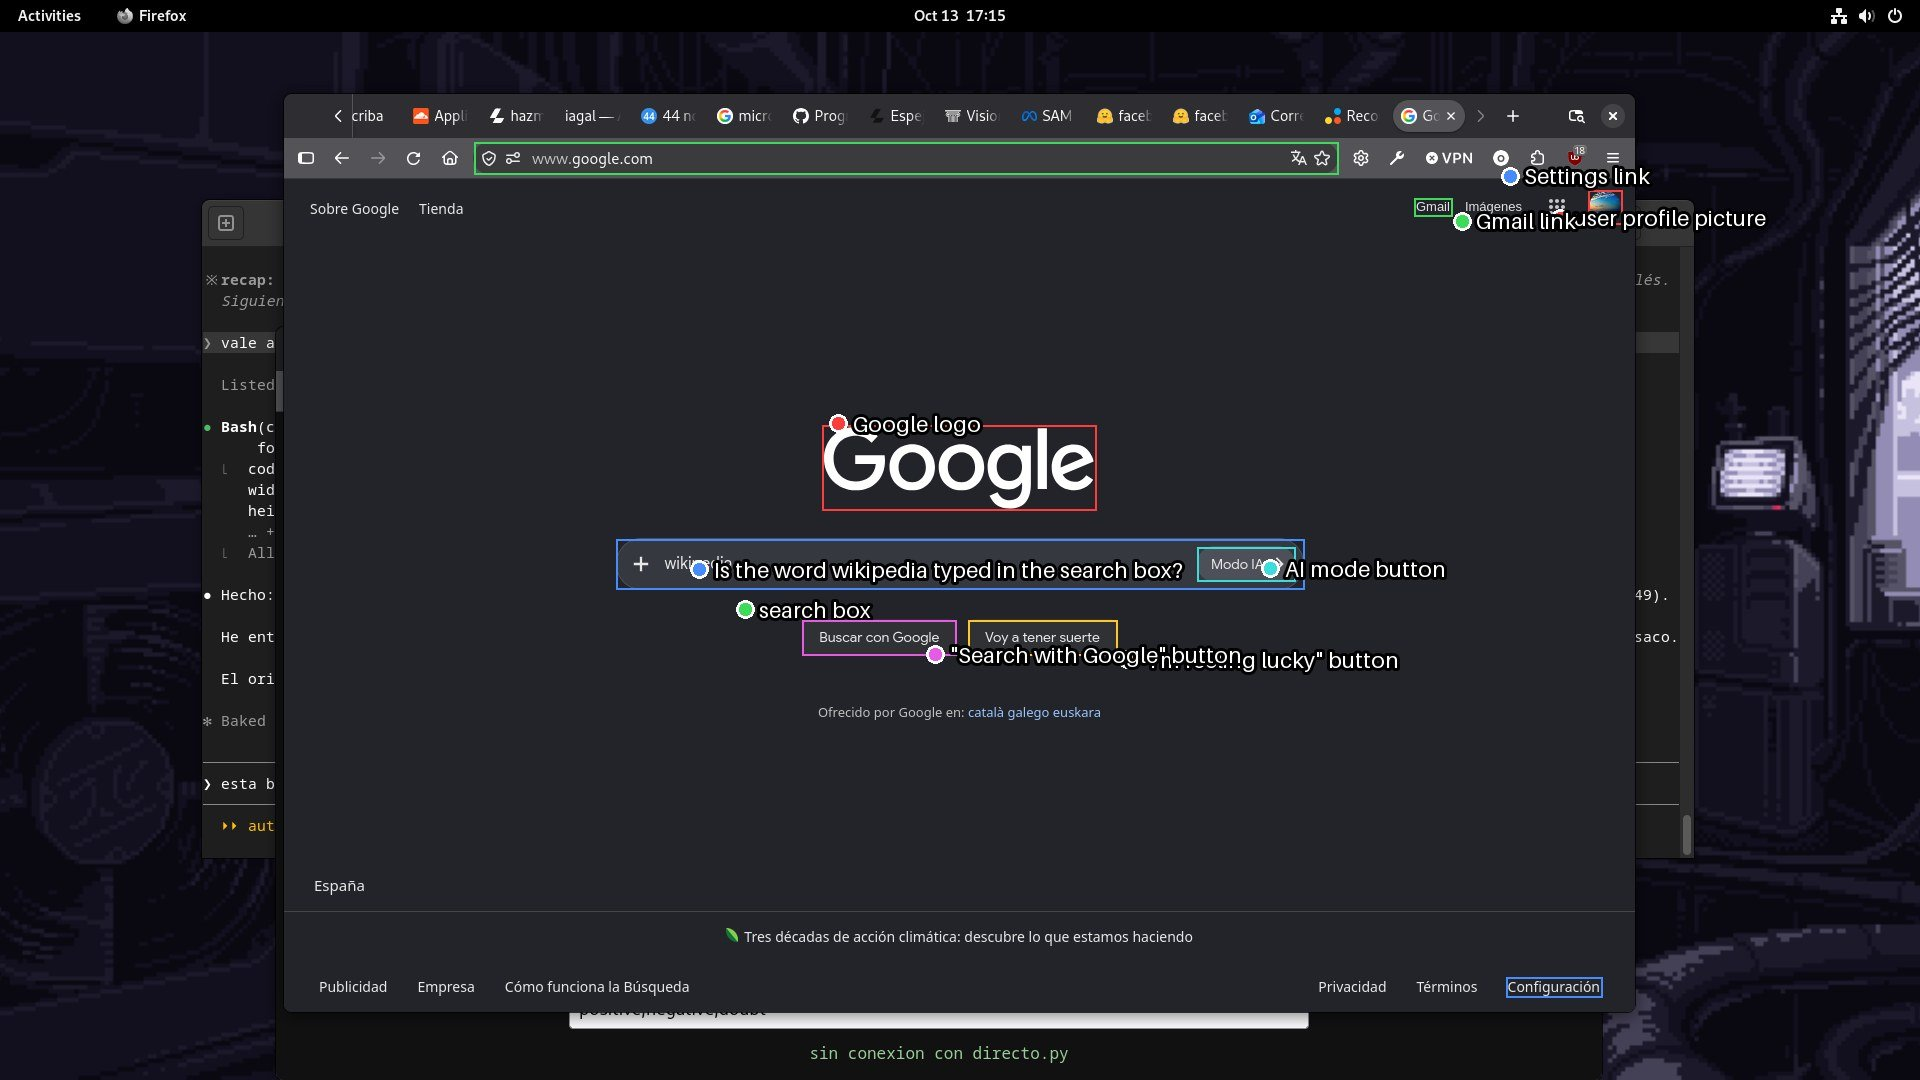
\includegraphics[width=0.495\textwidth]{figures/screen_google.jpg}\hfill
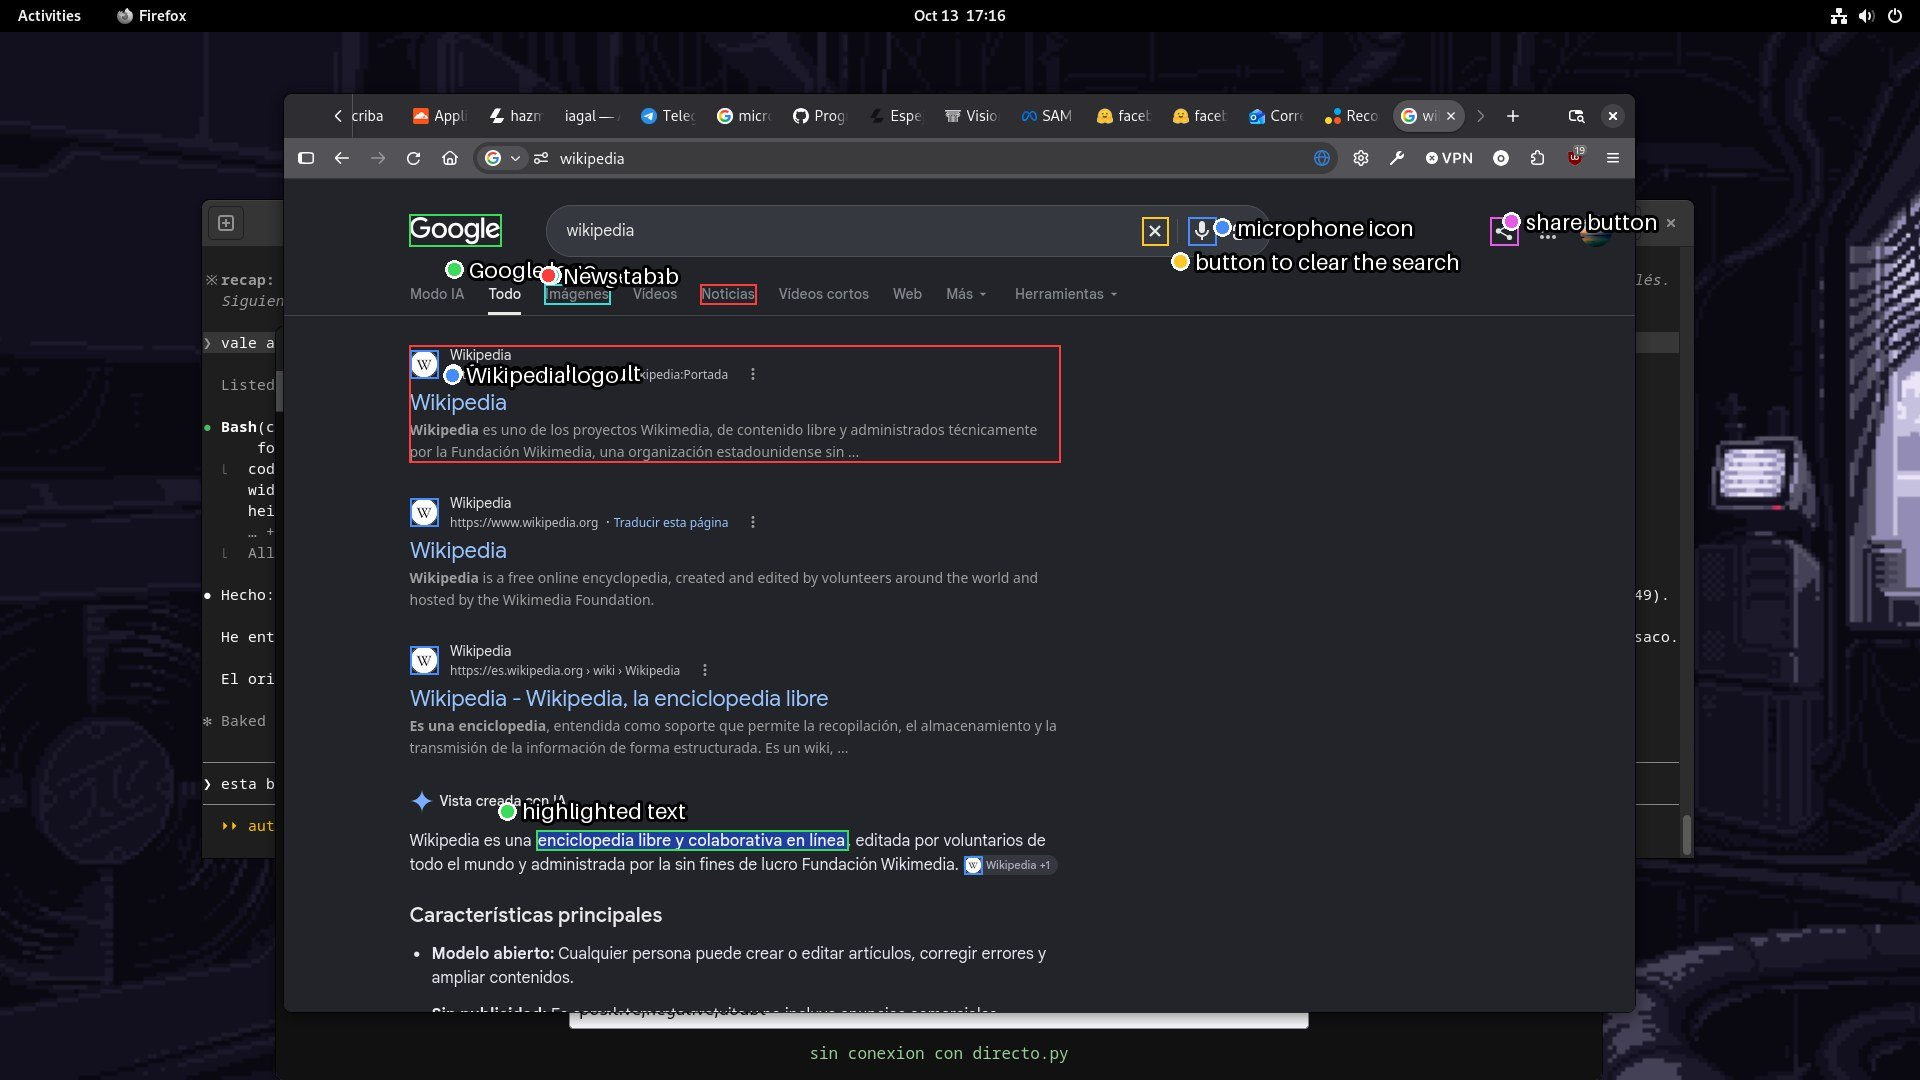
\includegraphics[width=0.495\textwidth]{figures/screen_results.jpg}
\caption{Two of the three screenshots at 1280 pixels. Rectangles are the
hand-drawn reference; the circle of the same colour is the attention peak for
that element. On these two, 16 of 18 present elements are affirmed, 5 points
fall inside the element and 16 within 40 pixels.}
\label{fig:screen}
\end{figure*}

\section{Discussion}

\textbf{The signal is real and cheap.} A model that was never trained to
localise carries, in five of its 1152 heads, a map that hits the object four
times out of five, and exposing it costs one extra short suffix per image. The
sink explains why naive attention roll-ups look uninformative, and dividing by
a content-free question removes it better than masking it.

\textbf{It is a point, not a detector.} One peak yields one object. Every
attempt to recover extent and multiplicity from the same map---thresholding,
several peaks, cleaning the segmenter's output---stays 25 points below a
segmenter that was trained to map a noun phrase to all its instances. On
named objects we see no reason to prefer the attention chain except speed
when scanning many classes.

\textbf{Deciding and delineating are different jobs.} The segmenter's score is
a poor judge of state, and the language model's attention is a poor
delineator. The combination we would build next uses the gap for the
condition and a segmenter for the extent, with the attention peak selecting
which instance the condition is about.

\textbf{Limitations.} The absent categories are random and therefore easy.
One category is asked per image and several instances count as one target, so
none of this is a detection benchmark, and no trained detector was run for
comparison. Localisation of predicates that are not object names rests on a
single photograph. The screenshot references were drawn by hand by the author.
The estimated per-concept cost of SAM 3 with a shared image encoding and the
end-to-end time of the hybrid on COCO were not measured separately. Only one
language model was dissected, and its head indices will not transfer.

\section{Conclusions}

A yes/no readout can be made to point: in Qwen3-VL-4B the decision is taken at
layer 24, the model looks at the image just before it, and five heads divided
by their response to a content-free question locate the object on 78.5\% of
held-out COCO images at no training cost and 12--17\,ms per additional
predicate. It cannot be made to segment competitively: SAM 3 given only the
word reaches 85.0\% of good boxes where the best point-prompted chain reaches
59.5\%. The useful system is therefore not a language model imitating a
detector but a language model judging predicates beside a segmenter that
delineates them, and the experiment that would establish its worth---pairs of
instances of one class that differ only in a state or relation---remains to be
run.

\section*{Code and data}

Code, experiment scripts, figures and this paper's sources are available at
\url{https://github.com/XxSamaxX/YOLOJ} under the MIT licence. The prompt
contract and readout come from SemIf \cite{semif} by way of \texttt{discern}
\cite{discern}. COCO images keep their original licences.

\bibliographystyle{plain}
\bibliography{refs}

\end{document}
